\vspace{-0.2cm}
\section{Experimental Evaluation}
\label{sec:eval}
\vspace{-0.2cm}
%
\begin{wrapfigure}{r}{0.35\textwidth}
    \centering
    \vspace{-0.45cm}
    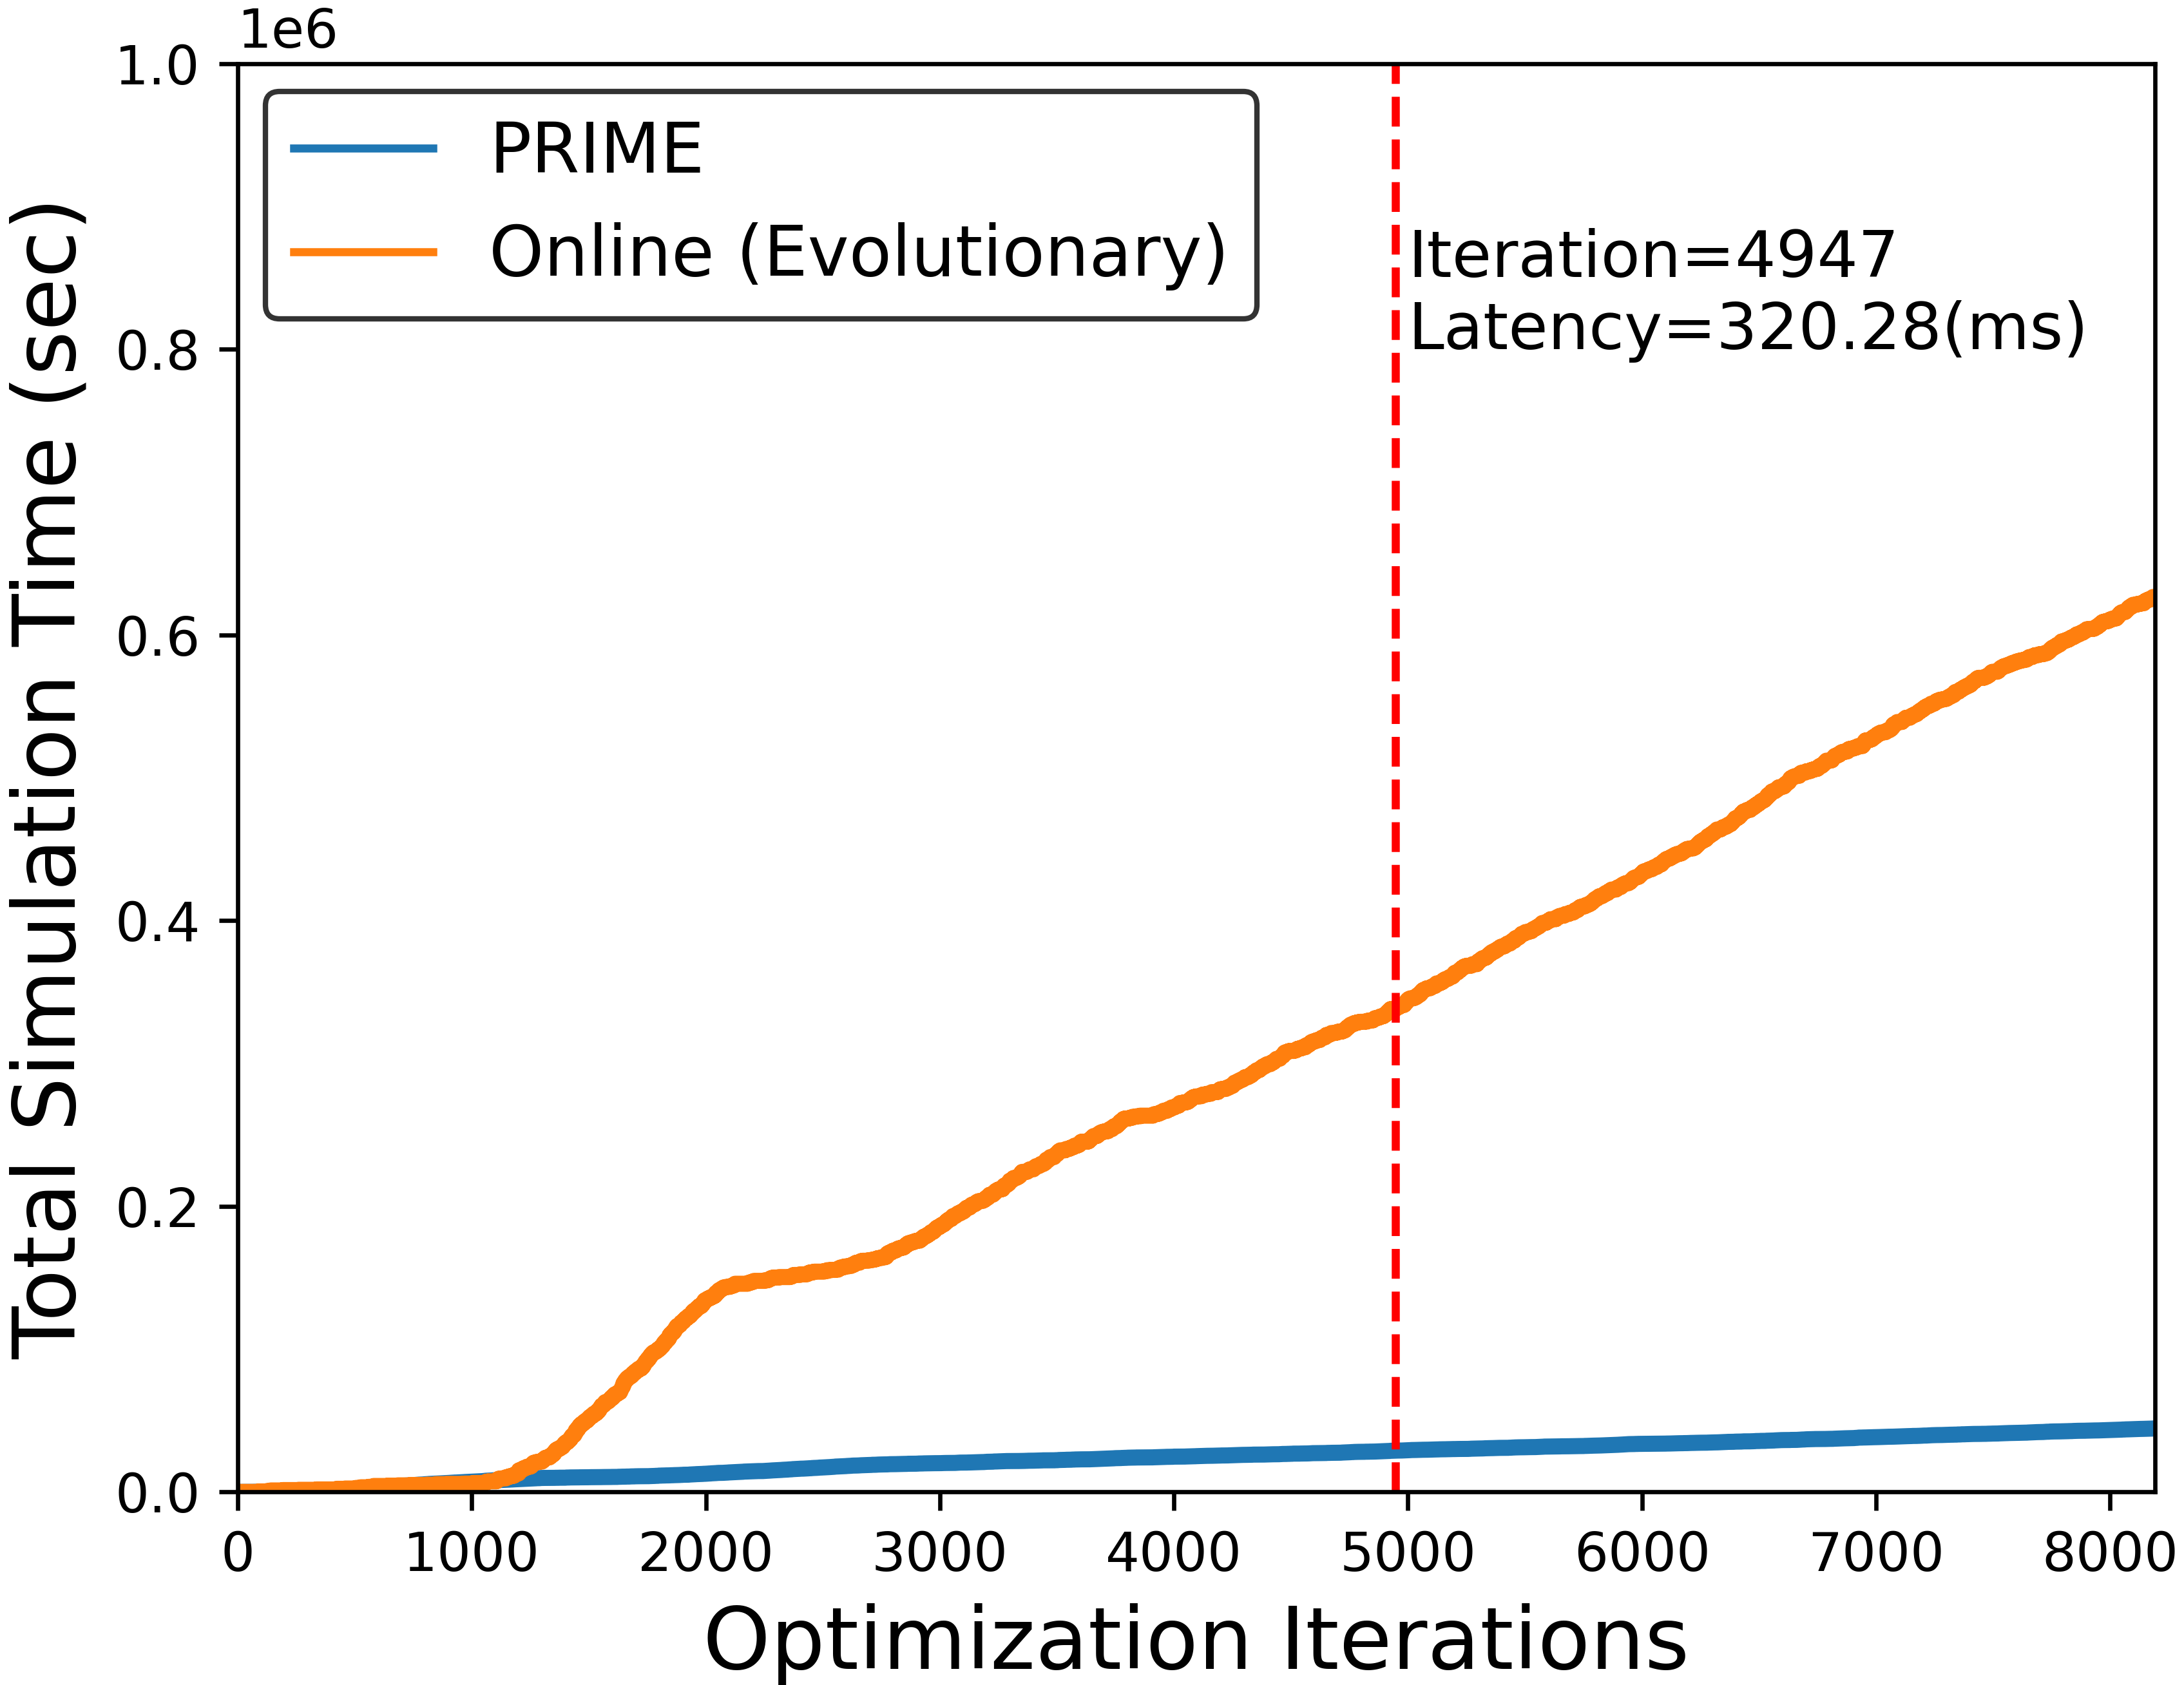
\includegraphics[width=0.98\linewidth]{chapters/prime/figs/motivation/simulation_time.png}
    \vspace{-0.3cm}
    \caption{\footnotesize{Comparing the total simulation time of \primemethodname\ (\review{for \primemethodname\ this is the total time for a forward-pass through the trained model on a CPU}) and evolutionary method on MobileNetEdgeTPU. \primemethodname\ only requires about \textbf{7\%} of the total simulation time of the online method.}}
    \vspace{-0.35cm}
    \label{fig:convergence_time}
\end{wrapfigure}
Our evaluations aim to answer the following questions: \textbf{Q(1)} {Can \primemethodname\ design accelerators tailored for a given application that are better than the best observed configuration in the training dataset, and comparable to or better than state-of-the-art simulation-driven methods under a given simulator-query budget?} \textbf{Q(2)} {Does \primemethodname\ reduce the total simulation time compared to other methods?} \textbf{Q(3)} {Can \primemethodname\ produce hardware accelerators for a family of different applications?} \textbf{Q(4)} {Can \primemethodname\ trained for a family of applications extrapolate to designing a high-performing accelerator for a new, unseen application, thereby enabling data reuse?} Additionally, we ablate various properties of \primemethodname\ (Appendix~\ref{sec:appx_ablation}) and evaluate its efficacy in designing accelerators with distinct dataflow architectures and a larger search space (up to 2.5$\times10^{114}$ candidates).

\niparagraph{Baselines and comparisons.}
%
We compare \primemethodname\ against three online optimization methods that actively query the simulator: \textbf{(1)} evolutionary search with the firefly optimizer~\citep{yazdanbakhsh2021apollo} (``Evolutionary''), which is the shown to outperform other online methods for accelerator design; \textbf{(2)} Bayesian Optimization (``Bayes Opt'')~\citep{vizier:sigkdd:2017},
\textbf{(3)} MBO~\citep{angermueller2019model}. 
%
%
In all the experiments, we grant all the methods the same number of feasible points. Note that our method do not get to select these points, and use the same exact offline points across all the runs, while the online methods can actively select which points to query, and therefore require new queries for every run. 
%
``$\mathcal{D}$(Best in Training)'' denotes the best latency value in the training dataset used in \primemethodname. We also present ablation results with different components of our method removed in Appendix~\ref{sec:appx_ablation}, where we observe that utilizing both infeasible points and negative sampling are generally important for attaining good results. 
%
Appendix~\ref{app:prime_additional_experiments} presents additional comparisons P3BO~\citep{p3bo:arxiv:2020}, a state-of-the-art method studied in the context of biological sequence design. 

\niparagraph{Architecting application-specific accelerators.}
%
We first evaluate \primemethodname\ in designing specialized accelerators for each of the applications in Table~\ref{tab:models}.
%
We train a conservative model using the method in Section~\ref{sec:prime_method} on the logged dataset for each application separately.
%
The area constraint $\alpha$ (Equation~\ref{eqn:opt_prob}) is set to $\alpha = 29~\text{mm}^2$, a realistic budget for accelerators~\citep{yazdanbakhsh2021apollo}. Table~\ref{table:results_single_task} summarizes the results.
%
On average, the best accelerators designed by \primemethodname\ outperforms the best accelerator configuration in the training dataset (last row Table~\ref{table:results_single_task}), by 2.46$\times$.
%
\begin{table*}[t!]
\small
\centering
\vspace*{0.1cm}
\caption{\label{table:results_single_task}Optimized objective values (i.e., latency in milliseconds) obtained by various methods for the task of learning accelerators specialized to a given application. Lower latency is better. \textbf{From left to right}: our method, online Bayesian optimization (``Bayes Opt''), online evolutionary algorithm (``Evolutionary''), and the best design in the training dataset. On average (last row), \methodname\ improves over the best in the dataset by 2.46$\times$ (up to 6.69$\times$ in t-RNN Dec) and outperforms best online optimization methods by 1.54$\times$ (up to 6.62$\times$ in t-RNN Enc). The best accelerator configurations identified is highlighted in bold.}
\resizebox{0.95\textwidth}{!}{% <------ Don't forget this %
\begin{tabular}{l|l|l|l|l|l}
\toprule
&&\multicolumn{3}{c|}{\textbf{Online Optimization}}&\\\cline{3-5}
\textbf{Application} & \textbf{\primemethodname} & \textbf{Bayes Opt} & \textbf{Evolutionary}&\textbf{MBO}&$\mathcal{D}$ \textbf{(Best in Training)}\\\midrule
{MobileNetEdgeTPU}&\textbf{298.50}&319.00&320.28&332.97&354.13\\\hline 
{MobileNetV2}&\textbf{207.43}&240.56&238.58&244.98&410.83\\\hline
{MobileNetV3}&\textbf{454.30}&534.15&501.27&535.34&938.41\\\hline
{\mfour}&\textbf{370.45}&396.36&383.58&405.60&779.98\\\hline
{\mfive}&208.21&201.59&\textbf{198.86}&219.53&449.38\\\hline
{\msix}&131.46&121.83&120.49&\textbf{119.56}&369.85\\\hline
{U-Net}&\textbf{740.27}&872.23&791.64&888.16&1333.18\\\hline
{t-RNN Dec}&\textbf{132.88}&771.11&770.93&771.70&890.22\\\hline
{t-RNN Enc}&\textbf{130.67}&865.07&865.07&866.28&584.70\\\bottomrule
\CC \textbf{Geomean of \primemethodname's Improvement}&\CC~1.0$\times$&\CC~\texttt{\textbf{1.58$\times$}}&\CC~\texttt{\textbf{1.54$\times$}}&\CC~\texttt{\textbf{1.61$\times$}}&\CC~\texttt{\textbf{2.46$\times$}}\\
\bottomrule
\end{tabular}% <------ Don't forget this %
}
\vspace{-0.1cm}
\end{table*} 
%
\primemethodname\ also outperforms the accelerators in the best online method by 1.54$\times$ (up to 5.80$\times$ and 6.62$\times$ in t-RNN Dec and t-RNN Enc, respectively).
%
Moreover, perhaps surprisingly, \primemethodname\ generates accelerators that are better than all the online optimization methods in 7/9 domains, and performs on par in several other scenarios (on average only 6.8$\%$ slowdown compared to the best accelerator with online methods in \mfive and \msix). 
%
These results indicates that offline optimization of accelerators using \primemethodname\ can be more data-efficient compared to online methods with active simulation queries.
%
To answer \textbf{Q(2)}, we compare the total simulation time of \primemethodname\ and the best evolutionary approach from Table~\ref{table:results_single_task} on the MobileNetEdgeTPU domain.
%
On average, not only that \primemethodname\ outperforms the best online method \review{that we evaluate}, but also considerably reduces the total simulation time by 93\%, as shown in Figure~\ref{fig:convergence_time}.
% 
Even the total simulation time to the first occurrence of the final design that is eventually returned by the online methods is about 11$\times$ what \primemethodname\ requires to fine a better design.
%
This indicates that data-driven \primemethodname\ is much more preferred in terms of the performance-time trade-off. \review{The fact that our offline approach \primemethodname\ outperforms the online evolutionary method (and also other state-of-the-art online MBO methods; see Table~\ref{table:p3bo_vs_prime}) is surprising, and we suspect this is because online methods get stuck early-on during optimization, while utilizing offline data allows us \primemethodname\ to find better solutions via generalization (see Appendix~\ref{app:online_opt_details}).} 


\begin{wrapfigure}{r}{0.35\textwidth}
    \centering
    \vspace{-0.7cm}
    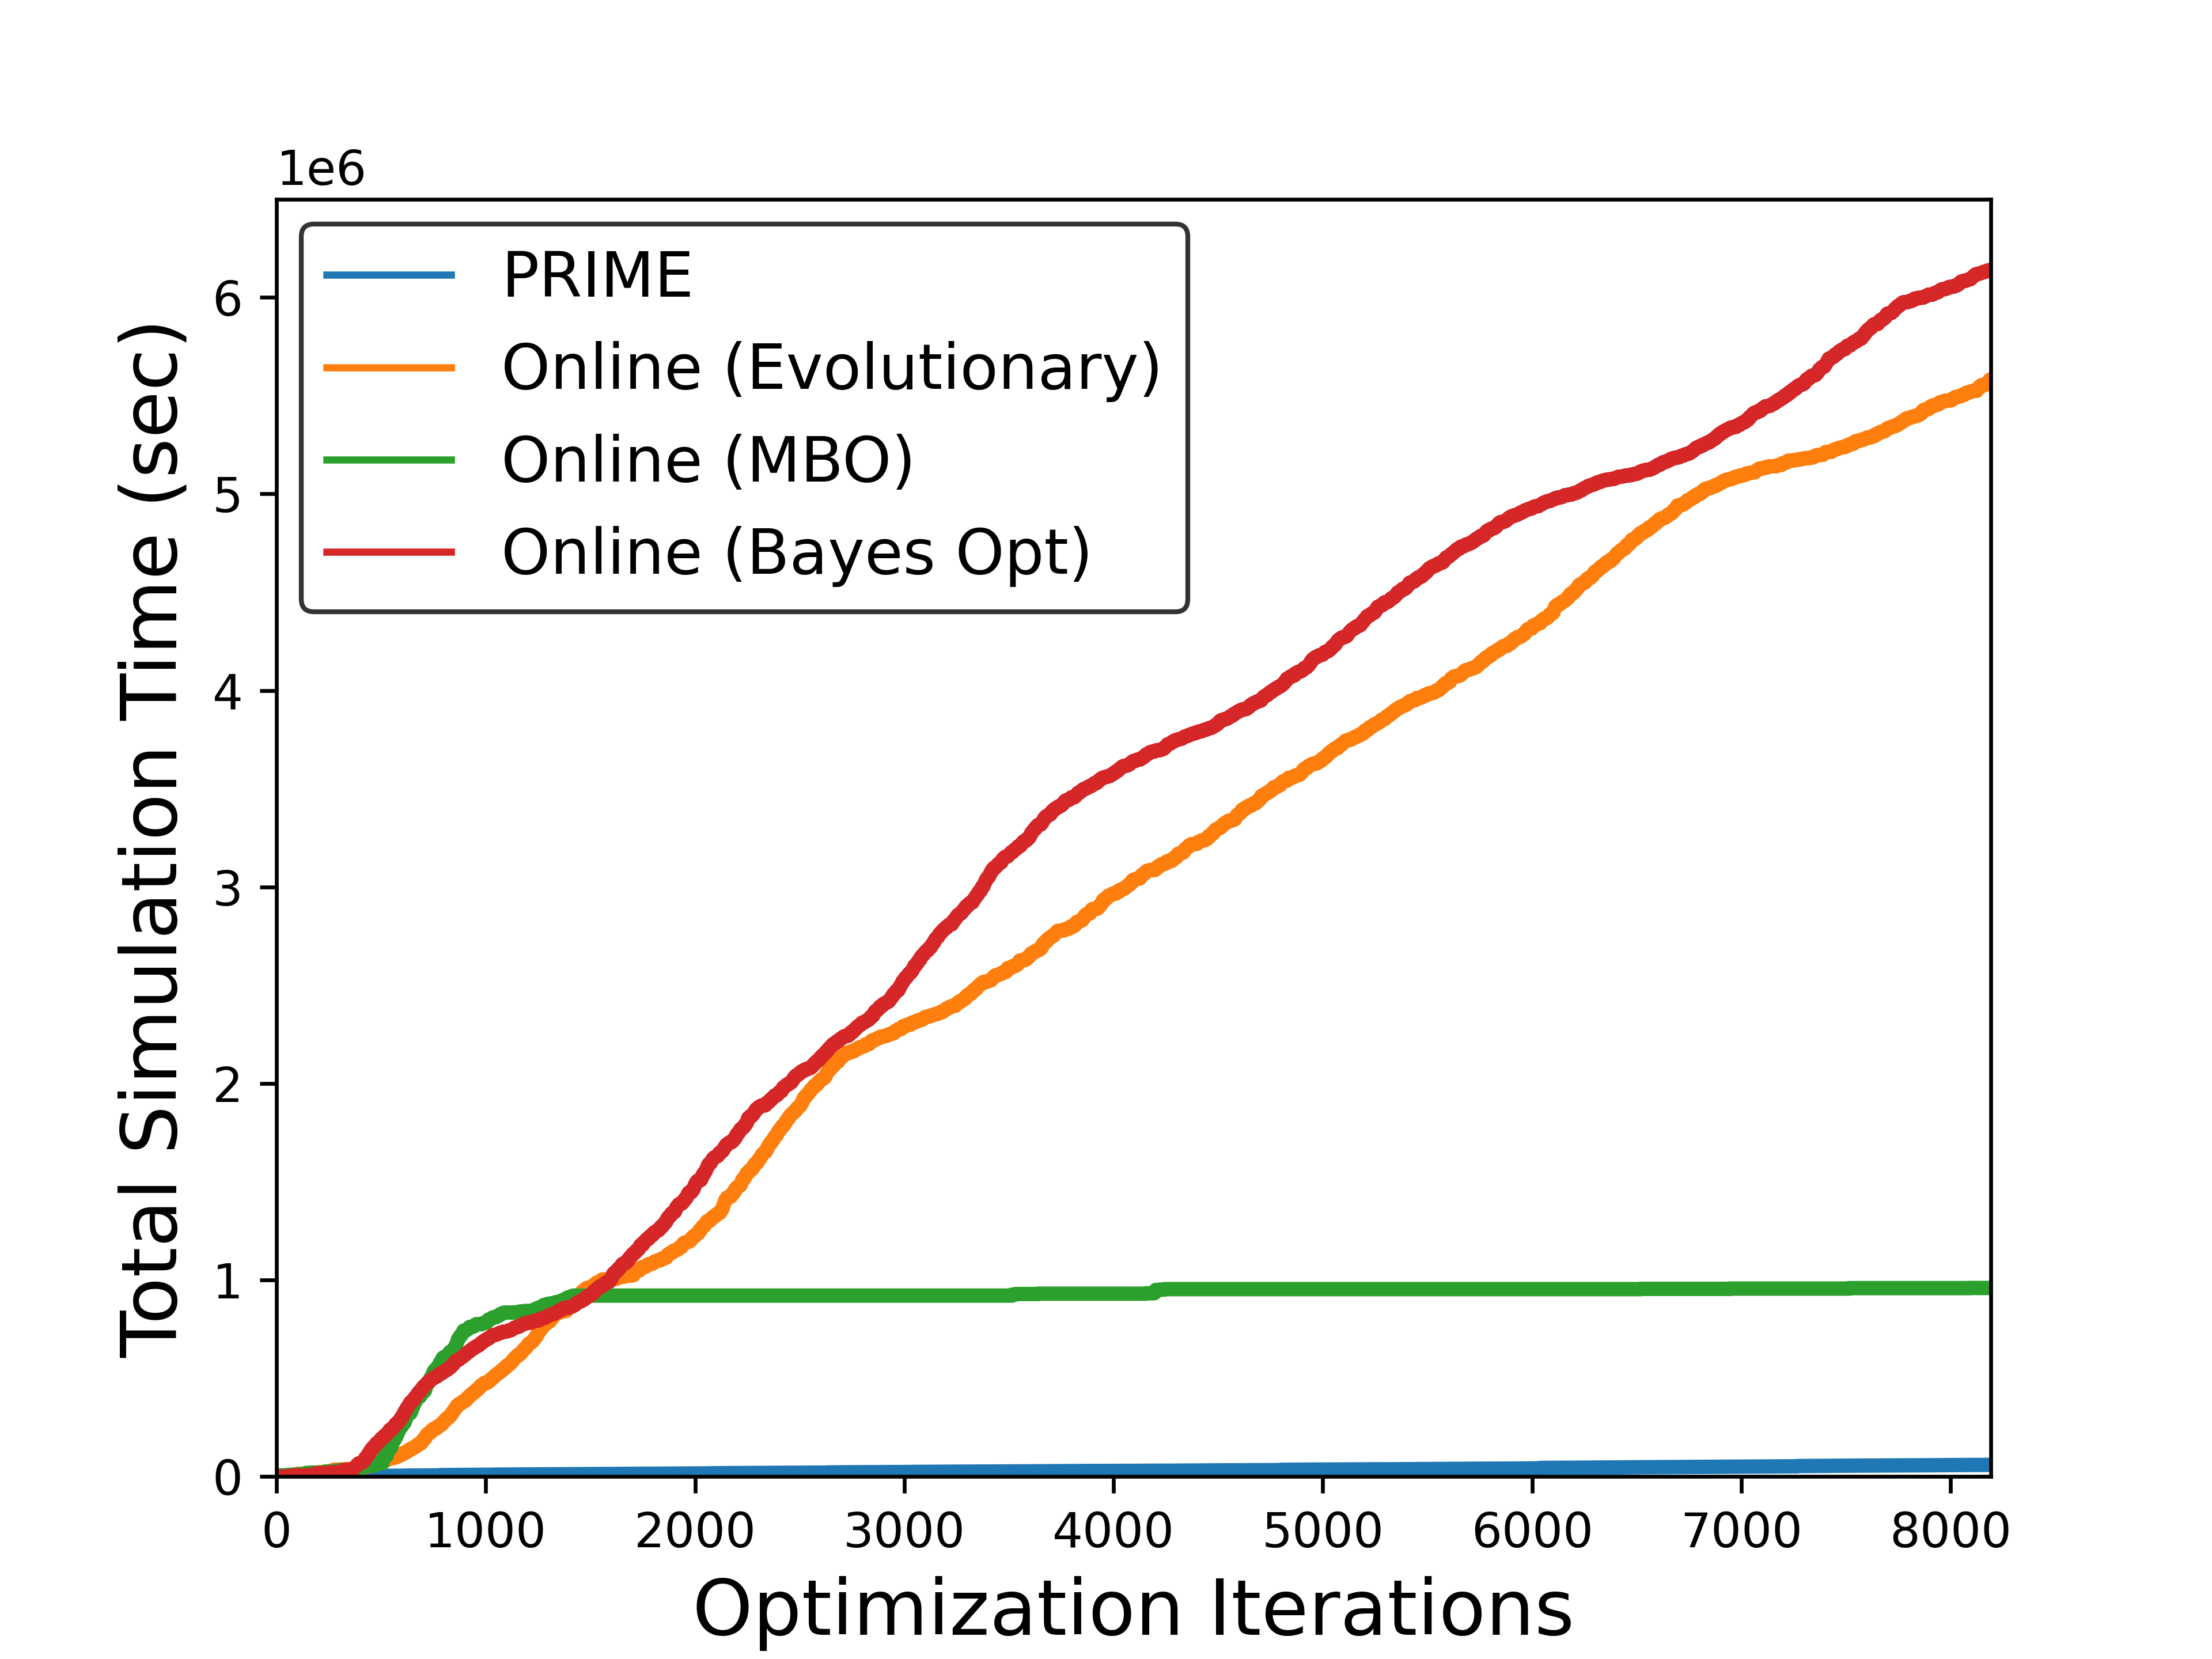
\includegraphics[width=0.98\linewidth]{chapters/prime/figs/motivation/convergence_time_seven_models.png}
    \vspace{-0.25cm}
    \caption{\footnotesize{Comparing the total simulation time needed by \primemethodname\ and online methods on seven models (Area $\leq$ 100mm$^2$)~. \primemethodname\ only requires about 1\%, 6\%, and 0.9\% of the total simulation time of Evolutionary, MBO, and Bayes Opt, respectively, although \primemethodname\ outperforms the best online method by 41\%.}}
    \vspace{-0.6cm}
    \label{fig:convergence_time_seven_models}
\end{wrapfigure}
\niparagraph{Architecting accelerators for multiple applications.}
%
To answer \textbf{Q(3)}, we evaluate the efficacy of the contextual version of \primemethodname\ in designing an accelerator that attains the lowest latency averaged over a set of application domains.
%
\begin{table*}[t!]
\small{
\centering
% \vspace*{0.1cm}
\caption{\label{table:results_multi_task} Optimized average latency (the lower, the better) across multiple applications (up to ten applications) for \primemethodname\ and best online algorithms (Evolutionary, MBO). Each row show the (Best, Median) of average latency across five runs. The geometric mean of \primemethodname's improvement over other methods (last row) indicates that \primemethodname\ is at least 21\% better.}
\vspace{-0.1cm}
\resizebox{\textwidth}{!}{\begin{tabular}{l|l|l|l|l}
\toprule
\textbf{Applications}&\textbf{Area}&\textbf{\primemethodname\ (Ours)}&\textbf{Evolutionary~ (Online)}&\textbf{MBO~(Online)}\\\midrule
% 3 Models
{MobileNet~(EdgeTPU, V2, V3)}&29~mm$^2$&(310.21, 334.70)&(\textbf{315.72}, \textbf{325.69})&(342.02, 351.92)\\\hline
% 4 Models
{MobileNet~(V2, V3), \mfive, \msix}&29~mm$^2$&(\textbf{268.47}, \textbf{271.25})
&(288.67, 288.68)&(295.21, 307.09)\\\hline
% 6 Models
{MobileNet~(EdgeTPU, V2, V3), \mfour, \mfive, \msix}&29~mm$^2$&(\textbf{311.39}, \textbf{313.76})&(314.31, 316.65)&(321.48, 339.27)\\\hline
% 7 Models
{MobileNet~(EdgeTPU, V2, V3), \mfour, \mfive, \msix, U-Net, t-RNN-Enc}&29~mm$^2$&\textbf{(305.47, 310.09)}&(404.06, 404.59)&(404.06, 412.90)\\\hline
{MobileNet~(EdgeTPU, V2, V3), \mfour, \mfive, \msix, t-RNN-Enc}&100~mm$^2$&\textbf{(286.45, 287.98)}&(404.25, 404.59)&(404.06, 404.94)\\\hline
% 9 Models
{MobileNet~(EdgeTPU, V2, V3), \mfour, \mfive, \msix, t-RNN~(Dec, Enc)}&29~mm$^2$&(\textbf{426.65}, \textbf{426.65})&(586.55, 586.55)&(626.62, 692.61)\\\hline
{MobileNet~(EdgeTPU, V2, V3), \mfour, \mfive, \msix, U-Net, t-RNN~(Dec, Enc)}&100~mm$^2$&(\textbf{383.57}, \textbf{385.56})&(518.58, 519.37)&(526.37, 530.99)\\\bottomrule
\CC \textbf{Geomean of \primemethodname's Improvement}&\CC~---&\CC~\texttt{\textbf{(1.0$\times$, 1.0$\times$)}}&\CC~\texttt{\textbf{(1.21$\times$, 1.20$\times$)}}&\CC~\texttt{\textbf{(1.24$\times$, 1.27$\times$)}}\\
\bottomrule
\end{tabular}}
}
\vspace{-0.2cm}
\end{table*}
%
As discussed previously, the training data used does not label a given accelerator with latency values corresponding to each application, and thus, \primemethodname\ must extrapolate accurately to estimate the latency of an accelerator for a context it is not paired with in the training dataset.
%
This also means that \primemethodname\ cannot simply return the accelerator with the best average latency and must run non-trivial optimization. 
%
We evaluate our method in seven different scenarios (Table~\ref{table:results_multi_task}), 
%
%
comprising various combinations of models from Table~\ref{tab:models} and under different area constraints, where the smallest set consists of the three MobileNet variants and the largest set consists of nine models from image classification, object detection, image segmentation, and speech recognition.
%
This scenario is also especially challenging for online methods since the number of jointly feasible designs is expected to drop significantly as more applications are added.
%
For instance, for the case of the MobileNet variants, the training dataset only consists of a few (20-30) accelerator configurations that are jointly feasible and high-performing (Appendix~\ref{sec:appx_multi_task_tsne}---Figure~\ref{fig:tsne_overlap}). 

Table~\ref{table:results_multi_task} shows that, on average, \primemethodname\ finds accelerators that outperform the best online method by 1.2$\times$ (up to 41\%).
%
While \primemethodname\ performs similar to online methods in the smallest three-model scenario (first row), it outperforms online methods as the number of applications increases and the set of applications become more diverse.
%
In addition, comparing with the best jointly feasible design point across the target applications, \primemethodname\ finds significantly better accelerators (3.95$\times$).
%
Finally, as the number of model increases the total simulation time difference between online methods and \primemethodname\ further widens (Figure~\ref{fig:convergence_time_seven_models}).
%
These results indicate that \primemethodname\ is effective in designing accelerators jointly optimized across multiple applications while reusing the same dataset as for the single-task, and scales more favorably than its simulation-driven counterparts.
%
Appendix~\ref{app:prime_analysis} expounds the details of the designed accelerators for nine applications, comparing our method and the best online method.


\niparagraph{Accelerating previously unseen applications (``zero-shot'' optimization).}
%
Finally, we answer \textbf{Q(4)} by demonstrating that our data-driven offline method, \primemethodname\ enables effective data reuse by using logged accelerator data from a set of applications to design an accelerator for an unseen new application, without requiring any training on data from the new unseen application(s).
%
We train a contextual version of \primemethodname\ using a set of ``training applications'' and then optimize an accelerator using the learned model with different contexts corresponding to ``test applications,'' without any additional query to the test application dataset.
%
Table~\ref{table:zero_shot} shows, on average, \primemethodname\ outperforms the best online method by 1.26$\times$ (up to 66$\%$) and only 2$\%$ slowdown in 1/4 cases.
%
Note that the difference in performance increases as the number of training applications increases.
%
These results show the effectiveness of \primemethodname\ in the zero-shot setting (more results in Appendix~\ref{sec:app_zero_shot}).

\niparagraph{Applying \primemethodname\ on other accelerator architectures and dataflows.}
%
Finally, to assess the the generalizability of \primemethodname\ to other accelerator architectures~\citep{kao2020confuciux}, we evaluate \primemethodname\ to optimize latency of two style of dataflow accelerators---NVDLA-style and ShiDianNao-style---across three applications (Appendix~\ref{sec:dla_shi_fast} details the methodology).
%
As shown in Table~\ref{table:dla_shi}, \primemethodname\ outperforms the online evolutionary method by 6\% and improves over the best point in the training dataset by 3.75$\times$.
%
This demonstrates the efficacy of \primemethodname\ with different dataflows and large design spaces.
%
\begin{table*}[t!]
\small
\centering
\vspace*{-0.1cm}
\caption{\label{table:zero_shot}Optimized objective values (i.e., latency in milliseconds) under zero-shot setting. Lower latency is better. From left to right: the applications used to train the surrogate model in \methodname\, the target applications for which the accelerator is optimized for, the area constraint of the accelerator, \methodname's (best, median) latency, and best online method's (best, median) latency. \methodname\ does not use any additional data from the target applications. On average (last row), \methodname\ yields optimized accelerator for target applications (with zero query to the target applications' dataset) with 1.26$\times$ (up to 1.66$\times$) lower latency over the best online method. The best accelerator configurations identified is highlighted in bold.}
\vspace{-0.1cm}
\resizebox{\textwidth}{!}{% <------ Don't forget this %
\begin{tabular}{l|l|l|l|l}
\toprule
\textbf{Train Applications}&\textbf{Test Applications}&\textbf{Area}&\textbf{\primemethodname\ (Ours)}&\textbf{Evolutionary~(Online)}\\\midrule
% Train = MobilenetEdge, MobilenetV3, Target = MobilenetV2
MobileNet~(EdgeTPU, V3)&{MobileNetV2}&29~mm$^2$&(\textbf{311.39}, \textbf{313.76})&(314.31, 316.65)\\\hline
MobileNet~(V2, V3), \mfive, \msix&{MobileNetEdge, \mfour}&29~mm$^2$&(357.05, 364.92)&(\textbf{354.59}, \textbf{357.29})\\\hline
MobileNet~(EdgeTPU, V2, V3), \mfour, \mfive, \msix, t-RNN Enc&{U-Net, t-RNN Dec}&29~mm$^2$&(\textbf{745.87}, \textbf{745.91})&(1075.91, 1127.64)\\\hline
MobileNet~(EdgeTPU, V2, V3),\mfour, \mfive, \msix, t-RNN Enc&{U-Net, t-RNN Dec}&100~mm$^2$&(\textbf{517.76}, \textbf{517.89})&(859.76, 861.69)\\\bottomrule
\CC \textbf{Geomean of \primemethodname's Improvement}&\CC---&\CC---&\CC~(1.0$\times$, 1.0$\times$)&\CC~(\texttt{\textbf{1.24$\times$}}, \texttt{\textbf{1.26$\times$}})\\
\bottomrule
\end{tabular}% <------ Don't forget this %
}
% \vspace{-0.1cm}
\end{table*}
\begin{table*}[t!]
\small
\centering
\renewcommand{\arraystretch}{1.1}
\vspace*{-0.05cm}
\caption{\label{table:dla_shi}Optimized objective values (i.e. total number of cycles) for two different dataflow architectures, NVDLA-style~\citep{nvdla} and ShiDianNao-style~\citep{shidiannao}, across three classes of applications. The maximum search space for the studied accelerators are $\approx$~2.5$\times$10$^{114}$. \primemethodname\ generalizes to other classes of accelerators with larger search space and outperforms the best online method by 1.06$\times$ and the best data seen in training by 3.75$\times$ (last column). The best accelerator configurations is highlighted in bold.}
\resizebox{0.95\textwidth}{!}{\begin{tabular}{l|l|l|l|l}
\toprule
\textbf{Applications}&\textbf{Dataflow}&\textbf{\primemethodname}&\textbf{Evolutionary ~(Online)}&\textbf{$\mathcal{D}$ (Best in Training)}\\\midrule
% MobileNetV2
MobileNetV2&NVDLA&\textbf{2.51$\times$10$^7$}&2.70$\times$10$^7$&1.32$\times$10$^8$\\\hline
MobileNetV2&ShiDianNao&\textbf{2.65$\times$10$^7$}&2.84$\times$10$^7$&1.27$\times$10$^8$\\\bottomrule
% ResNet50
ResNet50&NVDLA&\textbf{2.83$\times$10$^8$}&3.13$\times$10$^8$&1.63$\times$10$^9$\\\hline
ResNet50&ShiDianNao&\textbf{3.44$\times$10$^8$}&3.74$\times$10$^8$&2.05$\times$10$^9$\\\bottomrule
% Transformer
Transformer&NVDLA&\textbf{7.8$\times$10$^8$}&\textbf{7.8$\times$10$^8$}&1.3$\times$10$^9$\\\hline
Transformer&ShiDianNao&\textbf{7.8$\times$10$^8$}&\textbf{7.8$\times$10$^8$}&1.5$\times$10$^9$\\\bottomrule
\CC \textbf{Geomean of \primemethodname's Improvement}&\CC---&\CC~\texttt{\textbf{1.0$\times$}}&\CC~\texttt{\textbf{1.06$\times$}}&\CC~\texttt{\textbf{3.75$\times$}}\\
\bottomrule
\end{tabular}}
\vspace{-0.4cm}
\end{table*}